\chapter{Results}
\label{ch:results}

% sections
% 1 qualitative analysis (added by me)
% 2 setup
% 3 acquisition params
% 4 data treatment



% intro to results
This chapter presents the results of the thesis.
The results are divided into four parts: qualitative analysis of the spectra, characterization of the setup, optimization of the acquisition parameters, and data treatment.
As seen in the SE images presented in \cref{method:SE_images}, the areas chosen for the analysis are homogeneous and relatively clean.
Scratched areas on the GaSb specimen are shown in \cref{fig:SE_images:GaSb} panel (b), where some spectra were acquired, but not included in the results of this thesis.
% TODO discuss: the scratched areas behaved as expected, yielding poorer results than the homogeneous areas. ISO etc.



% 1 qualitative analysis
\section{Qualitative analysis}
\label{results:qualitative_analysis}

Here, an overview of the spectra is presented, where some characteristics and artifacts are identified, before addressing the setup parameters in \cref{results:setup}, acquisition parameters in \cref{results:acquisition_parameters}, and quantification results in \cref{results:data_treatment}.
General plots of the spectra are given in \cref{fig:results:overviewGaSb_withArtifacts,fig:results:GaSb_voltages,fig:results:GaAs_voltages}.



% figures/results/spectrum_overview.pdf
\begin{figure}[hbtp]
    \centering
    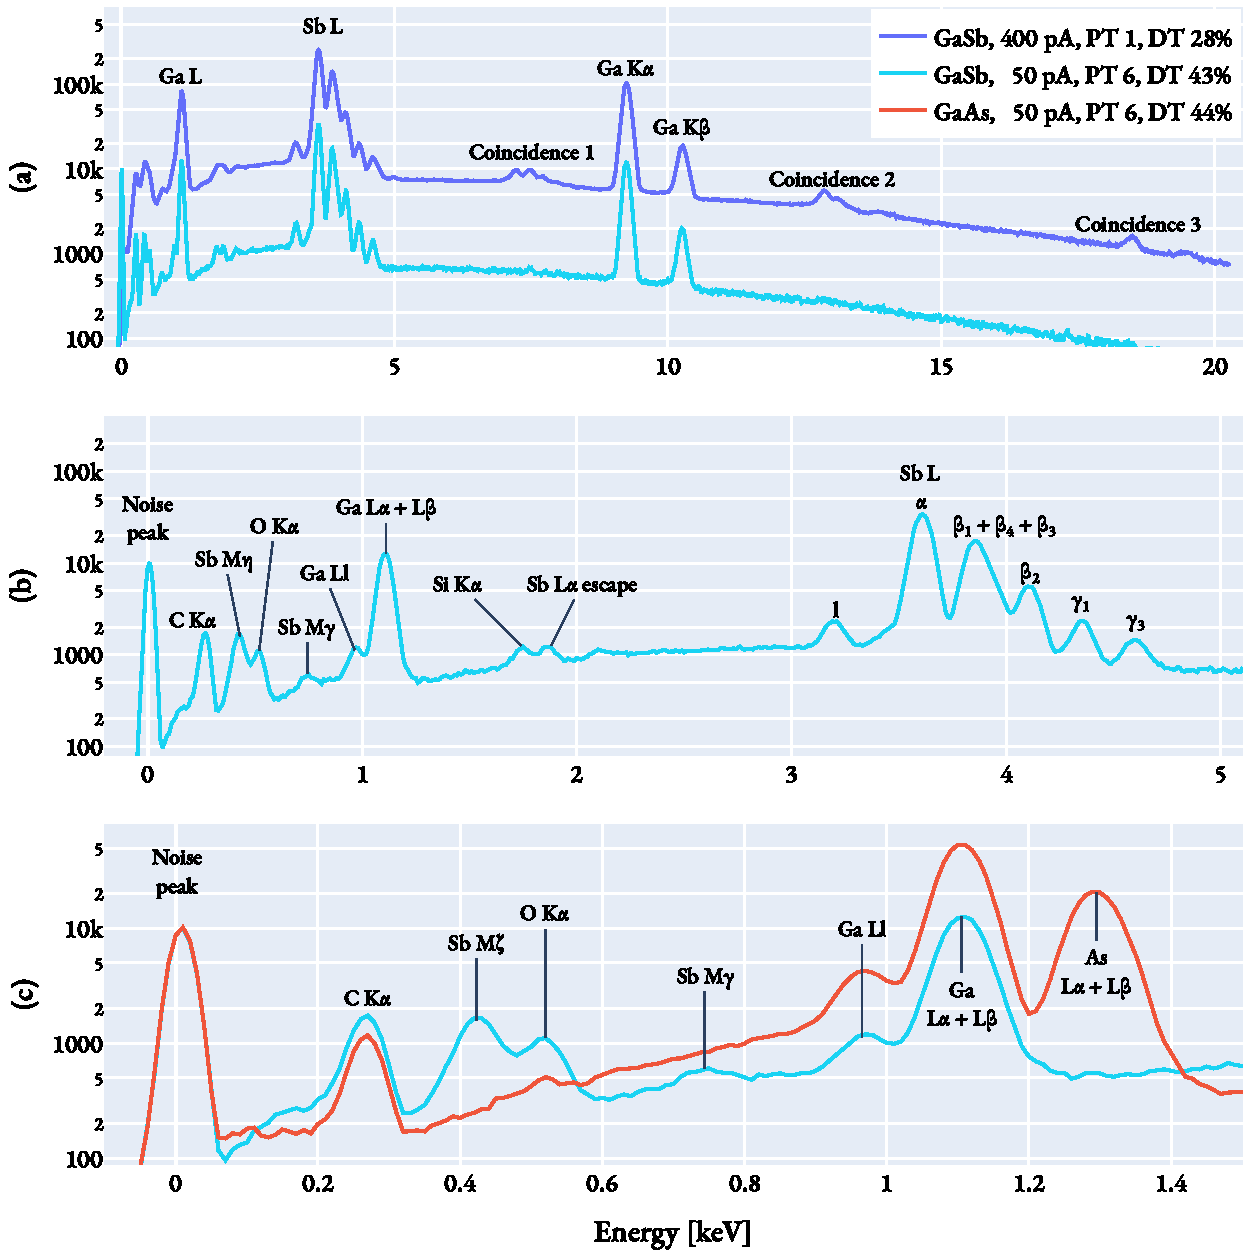
\includegraphics[width=0.99\linewidth]{figures/results/spectrum_overviews.pdf}
    \caption{
        Overview of the GaSb spectra.
        The blue line in panel (a) have lower resolution and more artifacts than the light blue line.
        The light blue line is plotted in panel (b) over a shorter energy range, and with peaks annotated.
        Panel (c) show the light blue line on an even shorter energy range, with the GaAs spectrum in red for reference.
        All three spectra are acquired with 30 kV.
    }
    \label{fig:results:overviewGaSb_withArtifacts}
\end{figure}


% figures/results/GaAs_voltages.pdf
\begin{figure}[hbtp]
    \centering
    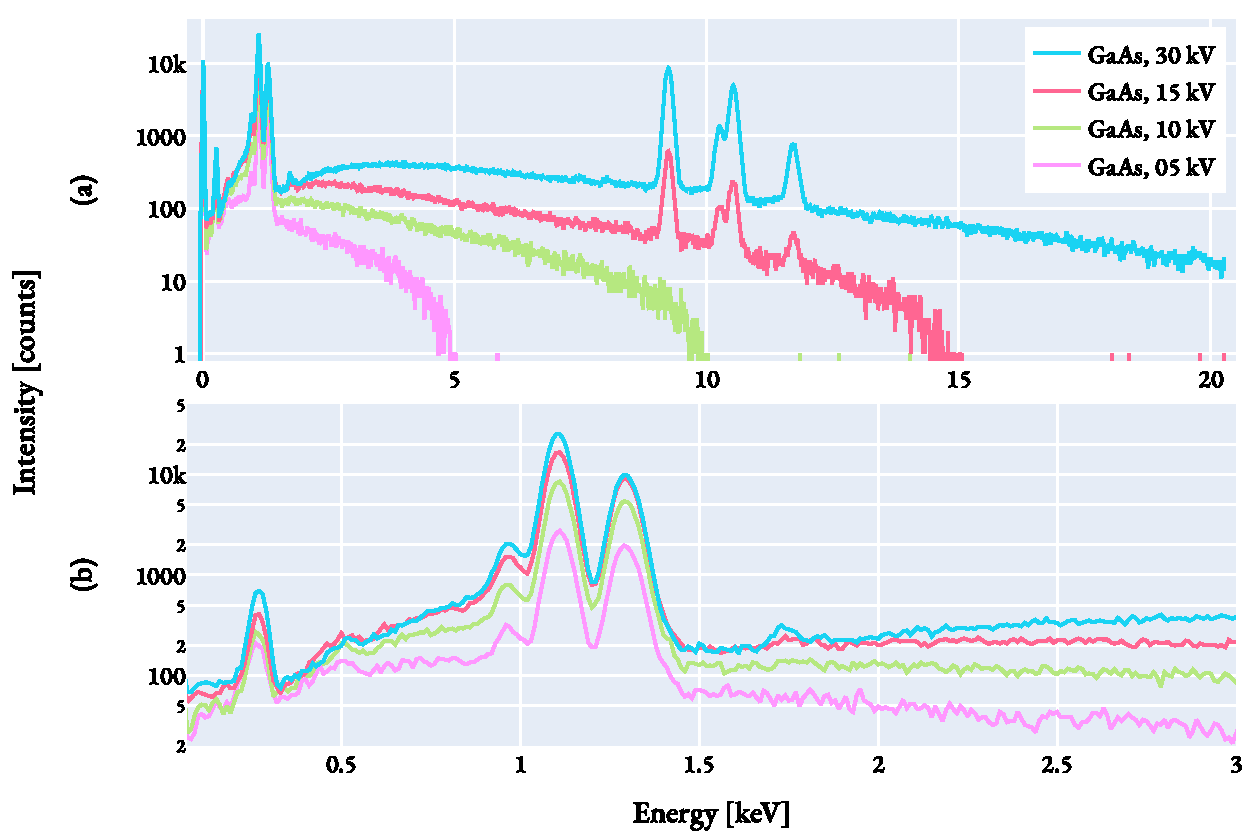
\includegraphics[width=0.85\linewidth]{figures/results/GaAs_voltages.pdf}
    \caption{
        Group (A), the GaAs voltage series.
        The figure gives an overview of the spectra, and show the effect of overvoltage.
        All four spectra have $i_b$ = 25 pA and PT 6.
    }
    \label{fig:results:GaAs_voltages}
\end{figure}


% figures/results/GaSb_voltages.pdf
\begin{figure}[hbtp]
    \centering
    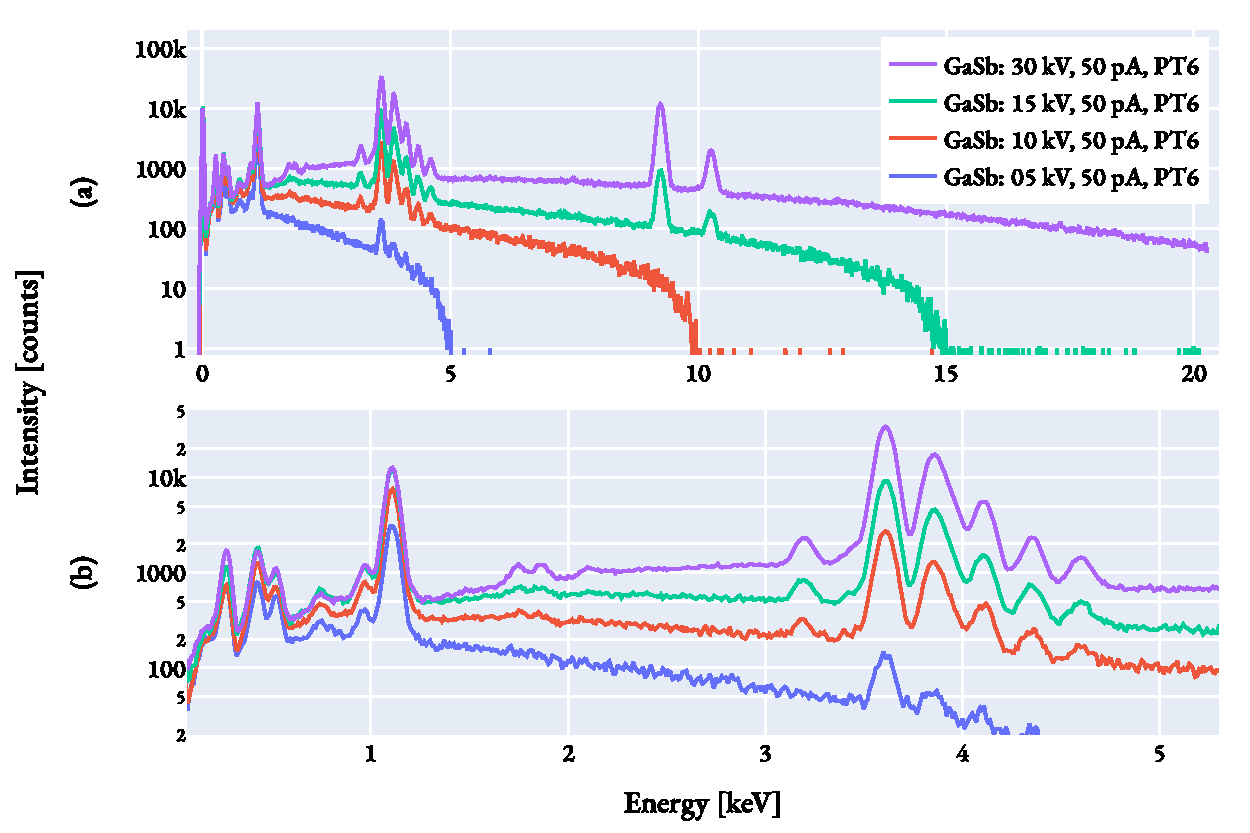
\includegraphics[width=0.85\linewidth]{figures/results/GaSb_voltages.pdf}
    \caption{
        Group (B), the GaSb voltage series.
        The figure serves the same purpose as \cref{fig:results:GaAs_voltages}, but for GaSb.
        % Additionally, an increased amound of coincidence counts compared to the GaAs spectra is visible in the tailing backgrounds, especially at 15 kV.
        The tailing background is the vertical lines above $E_0$.
        All four spectra have $i_b$ = 50 pA and PT 6.
    }
    \label{fig:results:GaSb_voltages}
\end{figure}





% \subsection*{Lines}
% \label{results:qualitative_analysis:lines}

All the lines given in \cref{tab:theory:lineEnergies} for Ga, As, and Sb have been identified in the spectra.
All spectra also had a peak at C K$\alpha$.
% TODO Ton: discus this C_Ka artifact, origin, in discussions
% TODO Ton: No other common peaks like Fe, or Si from set-up?
The GaSb spectra included a well defined O K$\alpha$ peak, while the GaAs spectra had barely any signal from the O K$\alpha$ line.
% TODO discuss: the O Ka peak might also be a Sb M-line, but I have not found the energy of the Sb M-lines.
As annotated in \cref{fig:results:overviewGaSb_withArtifacts}, the GaSb spectra also included two Sb M-signals: $\eta$ and $\gamma$, where $\eta$ is a clearly defined peak, while $\gamma$ is a slight increase in intensity.
These two M-peaks are not listed in the HyperSpy database, but were found through AZtec \cite{aztec_manual} and other literature \cite{liao2006practical}.
% TODO discuss: M lines are present in the absorption plot of GaSb



% \subsection*{Artifacts}
% \label{results:qualitative_analysis:artifacts}

Artifacts are present in all spectra, in varying degrees.
The artifacts identified are listed and described in \cref{tab:results:artifacts}.
The artifacts present in the spectra are the background, the noise peak, the carbon and oxygen stray peak, coincidence peaks, the internal Si fluorescence peak, and the Si escape peak from Sb La.

% The background is present in all spectra, and with increasing background intensity with higher count rates.
% The effect of a strong absorption edge which reduce the background intensity above its energy is most prominent in the GaAs spectra.
% Here it is the absorption edge in the L-peaks which reduce the background intensity abruptly above the L-peaks.
% Coincidence peaks are only present in some spectra, and are most prominent in the spectra with very high count rates.
% The spectra with beam energy 5, 10, and 15 keV also show coincidence events above $E_0$, e.g. visible in panel (a) in \cref{fig:results:GaSb_voltages}.


\begin{table}[phtb]
	\begin{center}
		\caption{
			The artifacts present in the spectra.
			See \cref{fig:results:overviewGaSb_withArtifacts,fig:results:GaSb_voltages,fig:results:GaAs_voltages}.
		}
		\renewcommand*{\arraystretch}{1.4}
		\label{tab:results:artifacts}
		\begin{tabular}{p{3.5cm}p{11.1cm}}
			\hline
			\textbf{Artifact}                                & \textbf{Where the articat is present and a comment}                                                                                                                                                                                                                                                                                                                                                                                             \\
			\hline
			Background                                       & All spectra. Increase with higher count rate.                                                                                                                                                                                                                                                                                                                                                                                                   \\
			Absorption edge effect on background             & Most prominent in GaAs. Reduces the background intensity above the Ga L absorption edge. In \cref{fig:results:GaAs_voltages} panel (b) the background drop from around 600 to around 170 counts.                                                                                                                                                                                                                                                \\
			Noise peak                                       & All spectra. Located almost at 0 keV.                                                                                                                                                                                                                                                                                                                                                                                                           \\
			Coincidence peaks                                & Only the spectra with very high count rates. \cref{fig:results:overviewGaSb_withArtifacts} with GaSb taken at 30 kV, 400 pA, and PT1 show coincidence peaks from: (Sb L + Sb L), (Sb L + Ga K), and (Ga K + Ga K).                                                                                                                                                                                                                              \\
			Tailing background noise from coincidence events & Present in spectra taken at 5, 10, and 15 kV. Coincidence events from two arbitrary counts give a tailing background. Exemplified by the green 15 kV line in \cref{fig:results:GaSb_voltages} panel (a), where vertical lines (one count each) are present between 15 and 20 keV.                                                                                                                                                               \\
			Internal fluorescence peak                       & Visible in some spectra. A low signal, barely a peak in some spectra, at Si K$\alpha$.                                                                                                                                                                                                                                                                                                                                                          \\
			Si escape peak                                   & Most GaSb spectra show some escape signal from Sb L$\alpha$ at 1.86 keV, labeled in \cref{fig:results:overviewGaSb_withArtifacts} panel (b). The coincidence counts from (Sb L + Sb L) marked as "Coincidence 1" in \cref{fig:results:overviewGaSb_withArtifacts} panel (a) has one peak at 7.2 keV and one at 7.5 keV, where the latter cound be a combination of coincidence events and escape counts from Ga K$\alpha$ (9.25 - 1.74 = 7.51). \\
			Stray C                                          & All spectra show a C K$\alpha$ peak, with some variation in intensity.                                                                                                                                                                                                                                                                                                                                                                          \\
			Stray O                                          & All spectra of GaSb show an O K$\alpha$ peak. The GaAs spectra have much lower, but still present signal at 0.52 keV.                                                                                                                                                                                                                                                                                                                           \\
			\hline
		\end{tabular}
	\end{center}
\end{table}



























% 2 setup
\section{Characterization of the setup}
\label{results:setup}

The parameters of the setup are: energy resolution, the energy scale and offset, peak ratios, and deviations in peak positions.
To show how the info in a single spectrum varies with the selected line of reference, information from the lines are presented from two selected spectra in \cref{tab:results:lines_info_30kV_50pA}.
The two selected spectra are both acquired with 30 kV, 50 pA, PT 6, DT 44\%, and ICR = 17k cps for GaSb and ICR = 16.5k cps for GaAs.
The table lists the theoretical energy of the line, the change in position after calibration, the FWHM of the peak, the area of the peak, the Fiori P/B of the line, and the estimated FWHM of Mn K$\alpha$ using \cref{eq:estimateFWHM}.


\begin{table}[phtb]
    \begin{center}
        \caption{
            Info from the lines acquired at 30 keV, 50 pA, and PT 6.
            The lines are sorted by area (counts in the peak).
            %The table lists the theoretical energy of the line, the change in position after calibration, the FWHM of the peak, the area of the peak, the Fiori P/B of the line, and the estimated FWHM of Mn K$\alpha$ using \cref{eq:estimateFWHM}.
            Both the GaAs and GaSb spectra have DT 44\%, with ICR = 17k cps for GaSb and ICR = 16.5k cps for GaAs.
        }
        \renewcommand*{\arraystretch}{1.4}
        \label{tab:results:lines_info_30kV_50pA}
        \begin{tabular}{llrlrrrp{2.5cm}}
            \hline
            \textbf{Specimen} & \textbf{Line} & \textbf{Energy} & \textbf{$\Delta$ E} & \textbf{FWHM} & \textbf{Area}     & \textbf{Fiori P/B} & \textbf{Estimated FWHM(Mn K$\alpha$)} \\
                              &               & \emph{[keV]}    & \emph{[eV]}         & \emph{[eV]}   & \emph{[k counts]} &                    & \emph{[eV]}                           \\
            \hline
                              & Ga L$\alpha$  & 1.098           & 2                   & 67            & 333               & 586                & 128                                   \\
                              & Ga K$\alpha$  & 9.252           & 2                   & 163           & 302               & 762                & 134                                   \\
                              & As K$\alpha$  & 10.544          & 2                   & 173           & 183               & 622                & 135                                   \\
            GaAs              & As L$\alpha$  & 1.282           & 2                   & 72            & 140               & 236                & 129                                   \\
                              & Ga L$\beta$   & 1.125           & 0                   & 68            & 56                & 97                 & 129                                   \\
                              & Ga K$\beta$   & 10.264          & 2                   & 161           & 39                & 124                & 123                                   \\
                              & As K$\beta$   & 11.726          & 2                   & 181           & 27                & 117                & 135                                   \\
                              & As L$\beta$   & 1.317           & 0                   & 71            & 23                & 39                 & 129                                   \\
            \hline
                              & Sb L$\alpha$  & 3.605           & -0.4                & 102           & 355               & 385                & 127                                   \\
                              & Ga K$\alpha$  & 9.252           & -2                  & 161           & 189               & 408                & 133                                   \\
            GaSb              & Sb L$\beta_1$  & 3.844           & -2                  & 101           & 152               & 168                & 124                                   \\
                              & Ga L$\alpha$  & 1.098           & 2                   & 65            & 74                & 86                 & 128                                   \\
                              & Sb L$\beta_2$  & 4.101           & 0                   & 108           & 55                & 63                 & 127                                   \\
                              & Ga K$\beta$   & 10.264          & -2                  & 160           & 24                & 59                 & 121                                   \\
            %&&&&&&&\\
            \hline
        \end{tabular}
    \end{center}
\end{table}



\subsection*{Energy resolution of the detector}
\label{results:setup:energy_resolution}

The energy resolution, as the estimated FWHM of the Mn K$\alpha$ peak, is both a function of the detector and certain acquisition parameters.
In the GaSb spectra the best energy resolution was 124 eV, obtained with PT 6, ICR = 22k cps, $E_0$ = 15 kV, and $i_b$ = 200 pA.
In the GaAs spectra the best energy resolution was 127 eV, obtained with PT 6, ICR = 880 cps, $E_0$ = 5 kV, and $i_b$ = 25 pA.
% TODO discuss: no obvious relation between the two best energy resolutions. But, it depends on the peaks in the spectrum.
% The best energy resolution obtained was: 124 eV for the GaSb spectra with PT 6, and 127 eV for the GaAs spectra.
The energy resolution should not be a function of the specimen, but as it is calculated with \cref{eq:estimateFWHM}, the outputted number depends somewhat on the peaks in the spectrum.
This is shown in \cref{tab:results:lines_info_30kV_50pA}, where the highest and lowest estimated energy resolution is 123 eV and 135 in the GaAs spectrum, and 121 eV and 133 eV in the GaSb spectrum.
% TODO discuss: Different peaks are used in GaSb and GaAs, thus we get different number with equal acquisition parameters.
% TODO discuss: Ga Kb gives the lowest, which might be a result of the overlap with As Ka.
The energy resolutions for all spectra are listed in \cref{tab:results:energy_resolutions}, with the relevant acquisition parameters.
These numbers for the energy resolution is calculated with HyperSpy, which have an issue explained in \cref{theory:eds_performance:energyres}.
As \cref{tab:results:energy_resolutions} shows, the energy resolution is affected by the two acquisition parameters: (i) process time and (ii) input count rate.
The ICR change with $E_0$ and $i_b$.
Specifying a single energy resolution for the detector should be accompanied by the acquisition parameters used to obtain that energy resolution.
Preferably, the value should also be an average with an uncertainty, calculated by several measurements with equal acquisition parameters.
This is not done here, but the values in \cref{tab:results:energy_resolutions} show that PT 6 give the best energy resolution at about 127 $\pm$ 2 eV.
When \cref{tab:results:lines_info_30kV_50pA} with the variations based on the peak of reference is taken into account, the energy resolution is more like 127 $\pm$ 6 eV.
% TODO discuss: The energy resolution is more like +- 6 eV, when we take into account the variations when using different peaks.



\begin{table}[htbp]
    \begin{center}
        \caption{
            The energy resolutions [eV] in the different spectra.
            The table is sorted by process time, then ICR.
            All energy resolutions are calculated with \cref{eq:estimateFWHM}.
        }
        % \renewcommand*{\arraystretch}{1.4}
        \label{tab:results:energy_resolutions}
        \begin{tabular}	{p{1.5cm}ccrrr}
            \hline
            \textbf{		} & \textbf{	Energy resolution	} & \textbf{	PT	} & \textbf{	ICR	} & \textbf{	E$_0$	} & \textbf{	I$_\textnormal{beam}$	} \\
            \hline
                        & 158                          & 1             & 17000          & 30               & 50                               \\
                        & 158                          & 1             & 160000         & 30               & 400                              \\
                        & 143                          & 2             & 17000          & 30               & 50                               \\
                        & 132                          & 4             & 17000          & 30               & 50                               \\
                        & 128                          & 6             & 1080           & 5                & 50                               \\
            GaSb        & 127                          & 6             & 2300           & 10               & 50                               \\
                        & 125                          & 6             & 5700           & 15               & 50                               \\
                        & 127                          & 6             & 17000          & 30               & 50                               \\
                        & 127                          & 6             & 17000          & 30               & 50                               \\
                        & 124                          & 6             & 22000          & 15               & 200                              \\
                        & 125                          & 6             & 42000          & 15               & 400                              \\
            \hline
                        & 127                          & 6             & 880            & 5                & 25                               \\
                        & 127                          & 6             & 1750           & 10               & 25                               \\
            GaAs        & 129                          & 6             & 3300           & 15               & 25                               \\
                        & 128                          & 6             & 8000           & 30               & 25                               \\
                        & 129                          & 6             & 16400          & 30               & 50                               \\
            \hline
        \end{tabular}
    \end{center}
\end{table}



\subsection*{Energy scale and offset}
\label{results:setup:scale_offset}

The energy scale and offset are the parameters which are used to calibrate the spectra.
Both metrics are quite consistent between the spectra, and the energy scale match with the setting used in the acquisition (10 eV per channel).
The averaged values and the standard deviations are listed in \cref{tab:results:scale_offset}.
The calculated scale of the detector is equal to the instrument setting at 10 eV per channel, with very low standard deviation between the spectra at 0.04 eV/channel.
The zero offset was calculated to be -0.205 keV, which is a deviation of half a channel from the instrument setting of -0.2 keV.
The standard deviation of the offset is 0.004 keV.

% TODO discuss: Comment that the std of the offset is one order of magnitude closer to the avg compared to the std vs avg of the scale.
% TODO discuss: why GaSb is slightly better std, might be because of the lines but also the higher i_b which gives more counts.

\begin{table}[htbp]
    \begin{center}
        \caption{
            The scale and offset in the spectra.
        }
        \renewcommand*{\arraystretch}{1.2}
        \label{tab:results:scale_offset}
        \begin{tabular}{rrrrr}
            \hline
            \textbf{Samples}   & \textbf{Scale, average} & \textbf{Scale, std}  & \textbf{Offset, average} & \textbf{Offset, std} \\
                               & \emph{[keV/channel]}    & \emph{[keV/channel]} & \emph{[keV]}             & \emph{[keV]}         \\
            \hline
            Instrument setting & 0.010000                & -                    & -0.2000                  & -                    \\

            GaSb               & 0.010001                & 8.7E-06              & -0.2044                  & 4.4E-03              \\
            GaAs               & 0.010018                & 6.6E-05              & -0.2075                  & 4.9E-03              \\
            GaSb + GaAs        & 0.010007                & 3.8E-05              & -0.2054                  & 4.3E-03              \\
            \hline
        \end{tabular}
    \end{center}
\end{table}




\subsection*{Peak ratios}
\label{results:setup:peak_ratios}

The results from the peak ratios are listed in \cref{tab:results:peak_ratios}.
The peak ratios are useful to alert carbon contamination over time, and to identify and quantify stray radiation with certain sample geometry.
As the results are neither a series over time or taken with the required sample geometry, the results in the table are a demonstration of the metric without any further interpretation.
Peak ratios are also used for quantification, but needs bulk corrections.
The table show that some of the peak ratios vary greatly with the acquisition parameters, e.g. the ratio between Ga L$\alpha$ and Sb L$\alpha$.


\begin{table}[phtb]
    \begin{center}
        \caption{
            Peak ratios calculated.
            The values varies with the beam energy, and thus the beam energies are grouped and an average is given with the corresponding standard deviation.
        }
        \renewcommand*{\arraystretch}{1.4}
        \label{tab:results:peak_ratios}
        \begin{tabular}{ccccl}
            \hline
            \textbf{Peaks}               & \textbf{$E_0$} & \textbf{Peak ratio} & \textbf{STD} & \textbf{Comment}              \\
            \hline
            Sb L$\alpha$ / Sb L$\beta_1$ & All            & 2.34                & 0            & Equal for all 11 GaSb spectra \\
            Ga L$\alpha$ / Sb L$\alpha$  & 5 kV           & 33.31               & -            & 1 GaSb spectrum               \\
            "                            & 10 kV          & 1.73                & -            & 1 GaSb spectra                \\
            "                            & 15 kV          & 0.76                & 0.008        & 3 GaSb spectra                \\
            "                            & 30 kV          & 0.21                & 0.004        & 6 GaSb spectra                \\
            Ga K$\alpha$ / Ga L$\alpha$  & 15 kV          & 0.19                & 0.0005       & 3 GaSb spectra                \\
            "                            & 15 kV          & 0.07                & -            & 1 GaAs spectrum               \\
            "                            & 30 kV          & 2.61                & 0.06         & 6 GaSb spectra                \\
            "                            & 30 kV          & 0.90                & 0.005        & 2 GaAs spectra                \\
            \hline
        \end{tabular}
    \end{center}
\end{table}



\brynjar{Eventually, take a new set of data to look at carbon contamination over time. Then make the table.}

\brynjar{TODO: redo these results. From ton: "yes, think is good to do. What
    would the advice be at the end? Take series or compare ratios for first and last
    spectrum to exclude C-contamination? For discussion: How does the measured ratio
    compare to the theoretical (quantum mechanics) ratio? And why?"}



\subsection*{Deviations in peak positions}
\label{results:setup:peak_positions}

No significant deviations in peak positions were observed.
The maximum deviation was 2 eV, and the minimum deviation was -2 eV, which is very low compared to the energy of the lines which are > 1 keV.



















% 3
\section{Optimization of the acquisition parameters}
\label{results:acquisition_parameters}

The performance metrics of the acquisition are: the Duane-Hunt limit, the Fiori peak-to-background ratio, and portion of counts in peaks vs background.
Additionally, results from the user parameters process time, beam energy, and beam current are presented.
The energy resolution is affected by both the detector and the acquisition setup, and the relevant results are presented in \cref{results:setup:energy_resolution}.



\subsection{Process time}
\label{results:process_time}

One of the parameters which was tested was the process time.
The process time is a trade-off between the energy resolution and the throughput.
This effect is illustrated in \cref{fig:results:energy_resolutions_process_time}, which is a plot of the GaSb spectrum at minimum and maximum process time.
Both spectra are taken at 30 kV with 50 pA.
The figure have three panels, (a) for low, (b) for medium, and (c) for high energy X-rays.
The effect of the lowered energy resolution is most prominent for the low energy X-rays.
The difference between the observable center of the peaks and the theoretical line energies in panel (a) is due to the poorer calibration at sub 1 keV energies.
In panel (a), the Sb M$\eta$ and O K$\alpha$ are merged together with PT 1, but are separated with PT 6.
The ability to seperate peaks is the definition of energy resolution, thus panel (a) is a good illustration of different energy resolutions.
The Ga L$l$ and Ga L$\alpha$ peaks are seperated with PT 6, but are merged together with PT 1.
With PT 4 (not shown), the Ga L$l$ and Ga L$\alpha$ peaks still seperated, but with PT 2 (not shown) they are merged together.
% TODO discuss: visible seperable and seperable with gaussian modelling is different. Visible seperable is important for qualitative analysis. And the quantitative is probably better with more seperated peaks, but overlapping can be dealt with quire well.
\cref{tab:results:energy_resolutions} show that the energy resolution with PT 1 is 158 eV, and with PT6 it is 127 eV.
In panel (b) with the medium energies, the contrast of the peaks are lowered, i.e. the difference between the top of the peaks and the valley between the peaks are lowered.
The effect of the lowered energy resolution is not as prominent panel (c) for high energy X-rays.

% TODO discuss: for high energies the peaks are also well seperated.


% figures eds_energyResolutions_process_time.pdf
\begin{figure}[hptb]
    \centering
    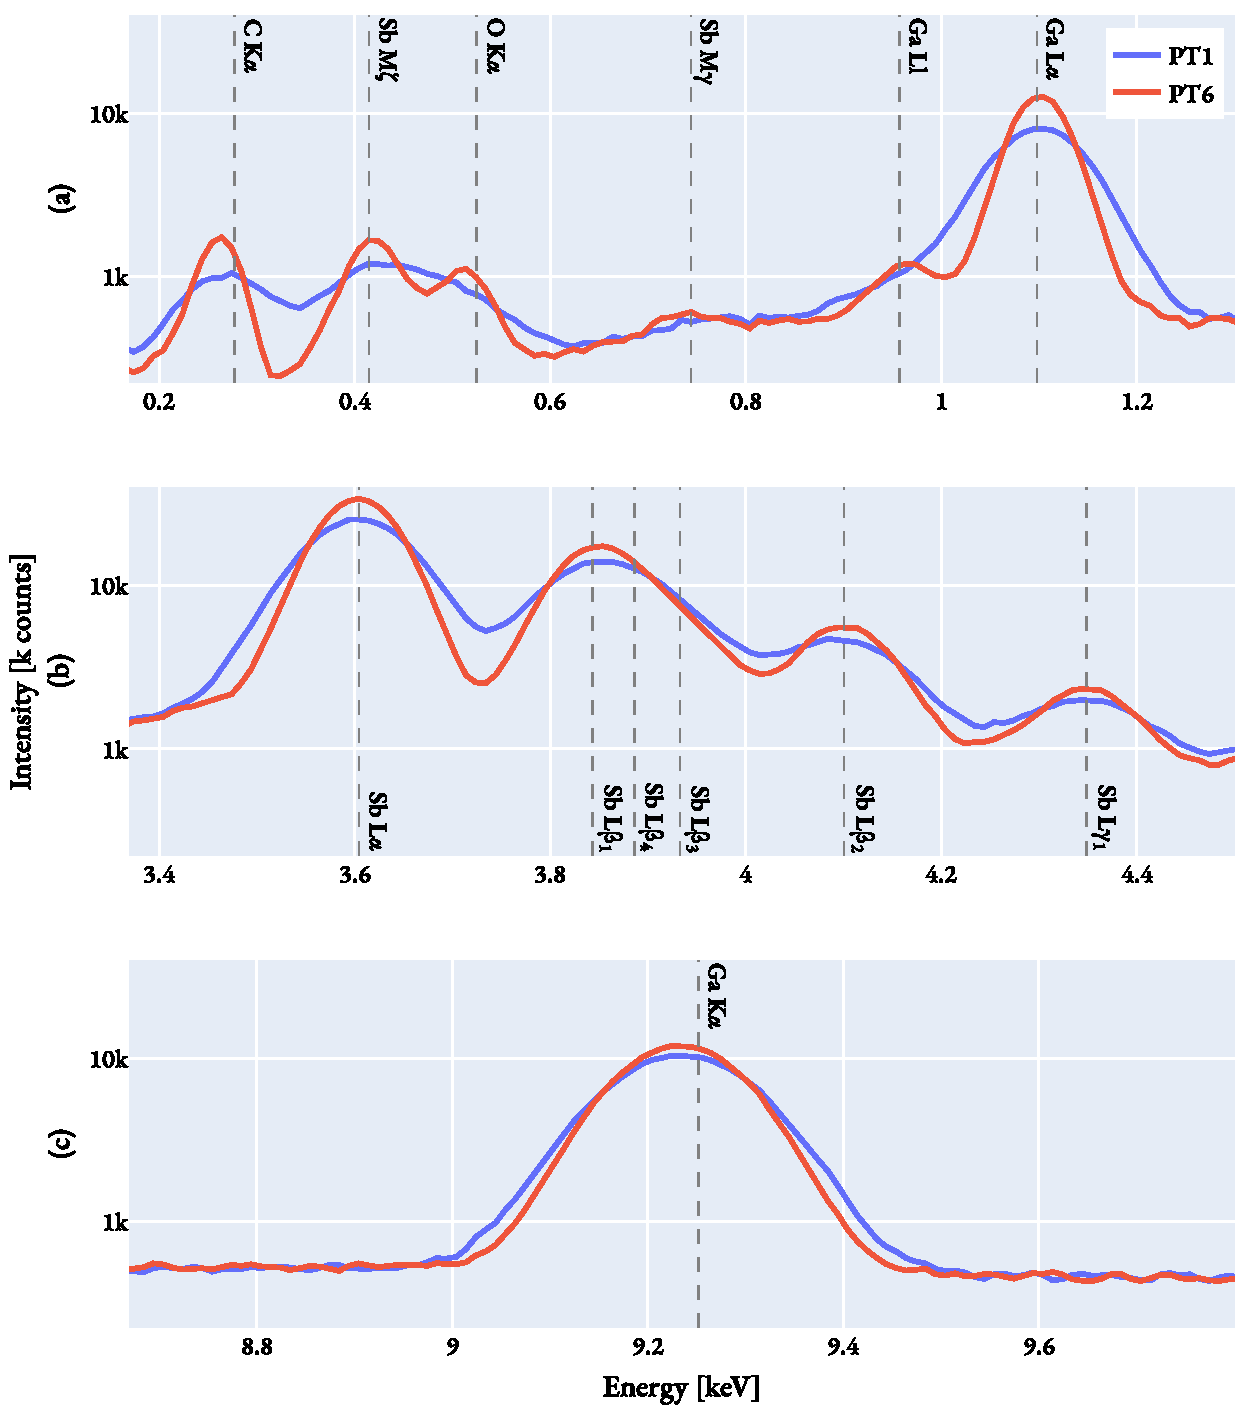
\includegraphics[width=0.95\linewidth]{figures/results/eds_energyResolutions_process_time.pdf}
    \caption{
        Different energy resolutions on the same specimen, because of different process times.
        The maximum (red) and minimum (blue) PT on the instrument is used.
        $E_0$ = 30 kV, $I_b$ = 50 pA for both spectra.
        The PT 1 and PT 4 spectra are not shown, but are in between the PT 2 and PT 6 spectra.
        Panel (a) is the spectrum at low energy, where the effect most influential.
        With PT 1 the Sb M$\eta$ and O K$\alpha$ peak are merged, and the Ga L$l$ and Ga L$\alpha$ peaks are merged.
        Panel (b) is the spectrum at medium energy, where the effect less influential, but the peak contrast is lowered.
        Panel (c) is the spectrum at high energy, where the effect is almost negligible.
        All three panels span 1.13 keV and have the same range of counts.
        The vertical lines are the theoretical line energies.
    }
    \label{fig:results:energy_resolutions_process_time}
\end{figure}


The effect of the process time on the FWHM of the lines is shown in \cref{tab:results:PTvsFWHMs}.
The table shows the measured FWHM of Ga L$\alpha$, Sb L$\alpha$, and Ga K$\alpha$ for different process times.
The measurement is done on the Gaussian fit of the peaks.
Additionally, the FWHM of the Mn K$\alpha$ is estimated for each process time.
The table shows the variations on the GaSb specimen with PT 1, 2, 4, and 6.
The last row shows the FWHM in the GaAs specimen at PT 6 for reference.
All spectra in the table were acquired at 30 kV and 50 pA.
In the GaSb spectra, the PT 1 has DT 4\%, PT 2 has DT 7\%, PT 4 has DT 13\%, and PT 6 has DT 44\%.
The GaAs spectrum with PT 6 has DT 44\%.

% TODO discuss: based on the numbers, PT 4 should be good enough for most applications. High resolution, and much faster than PT 6. DT44 is really high, and not nice for mapping.
% TODO discuss: specimen with many L-lines


\begin{table}[phtb]
    \begin{center}
        \caption{
            FWHMs of lines with different process times.
            All the FWHMs are in eV, calculated from the Gaussian fit.
            All spectra are acquired at 30 kV and 50 pA.
            GaSb is used as the specimen, except for the last column, where GaAs is used for reference.
        }
        \renewcommand*{\arraystretch}{1.4}
        \label{tab:results:PTvsFWHMs}
        \begin{tabular}{rrrrrr}
            \hline
            \textbf{Line}       & \textbf{PT 1} & \textbf{PT 2} & \textbf{PT 4} & \textbf{PT 6} & \textbf{PT 6, GaAs} \\
            \hline
            %C K$\alpha$&&&&&\\ % C is not it the models used
            Ga L$\alpha$        & 109           & 88            & 73            & 65            & 67                  \\
            Sb L$\alpha$        & 138           & 122           & 108           & 102           & -                   \\
            Mn K$\alpha$ (est.) & 158           & 143           & 132           & 127           & 129                 \\
            Ga K$\alpha$        & 182           & 172           & 165           & 161           & 163                 \\
            \hline
        \end{tabular}
    \end{center}
\end{table}



\subsection{Beam energy and beam current}
\label{results:beam_energy_and_beam_current}


% comment on (A) and (B)
The energy and the amount of electrons in the probe is important for the emerging X-ray spectrum.
Using a low overvoltage is both problematic for the qualitative and quantitative analysis.
The green line in \cref{fig:results:GaAs_voltages} is the 10 kV spectrum for GaAs, which has no visible signal from the Ga K$\alpha$ peak, where the overvoltage is around 1.1.
The overvoltage is also an issue for the Sb L-lines in the 5 kV spectrum in \cref{fig:results:GaSb_voltages}.
The Sb L-peaks are present, but weak, and the L$l$ peak is not visible.
This issue with the weak Sb-L peaks makes the quantification of Sb difficult at low voltages, as seen further down in \cref{results:initial_quantification}.
The GaAs specimen is quantified much more accurately at 5 kV, beacuse the Ga L$\alpha$ and As L$\alpha$ peaks have similar overvoltages.
In the voltage series, which are group (A) and (B) in \cref{method:acquisition_settings}, the amount of counts in the lower voltages are quite low.
The low amount of counts is due to keeping the beam current constant at 50 and 25 pA.
Using a higher beam current on the lower energies would have made normalization more necessary, which is adding a layer of subjective decisions as the spectra must be normalized to something.
% TODO discuss: this might not have been the best choice. For future work one can try to get the same ICR for all voltages, and see if the results are better and still comparable, without normalization.
Even though the 30 kV spectra in GaAs and GaSb have more counts and are smoother than the other spectra, they both have more artifacts.
% TODO discuss: the amount of artifacts have to be adjusted for the specimen and the goal of the analysis.
Around 1 keV, the 30 kV and 15 kV spectra are quite similar.
% TODO discuss: at 1 keV, the ionization cross section when using 15 or 30 kV is more or less the same.

\brynjar{TODO: write something about ICR?}

% (C) (D) and (E)
As the 30 and 15 kV spectra gave better results for GaSb, they were chosen for group (C), (D), and (E).
In (C) different process times were tested, and these results are presented in \cref{results:process_time}.
In (D) different beam currents were tested, while also changing the PT and $E_0$.
In (E) the data type maps were acquired.
% (D)
The combination of high $i_b$ and high PT in two of the spectra in (D) made the DT very high.
Despite the high DT, the amount of artifacts in the 200 pA and 400 pA spectra were similar to the 50 pA spectra.
However, with DT at 53\% and 77\%, the acquisition time was very long.
% TODO discuss: DT is not a good measure of the artifacts, at least not when using high PT which allows the electronics to count accurately. However, high i_b and PT is bad for mapping.
On the quantification presented in \cref{results:initial_quantification}, the beam energy appears to be more important than the beam current.
% TODO discuss: this might be a result of the lines used (Ga L or Ga K).
\brynjar{TODO: the maps have not been alalysed properly yet.}








\subsection{Duane-Hunt limit}
\label{results:duane_hunt}

The Duane-Hunt limits, or the effective beam energies, are presented in \cref{tab:results:duane_hunt}.
The table shows the Duane-Hunt limit for the 5, 10, and 15 kV spectra.
As the energy range recorded in the spectra were 0-20 keV, the Duane-Hunt limit of the 30 kV spectra were not possible to calculate.
All the calculated Duane-Hunt limits are within 0.2 keV of the nominal beam energy, i.e. the specified beam energy in the SEM software.
The average deviation is 0.06 keV, with a standard deviation of 0.04 keV.
This shows that the beam energy is quite stable.
% TODO discuss: the usefulness of calculating the DH limit.

\begin{table}[htbp]
    \begin{center}
        \caption{
            The Duane-Hunt limit in the sub 30 kV spectra.
            All spectra are acquired with PT 6.
        }
        % \renewcommand*{\arraystretch}{1.4}
        \label{tab:results:duane_hunt}
        \begin{tabular}{rrrrr}
            \hline
            \textbf{Group} & \textbf{Specimen} & \textbf{$E_0$} & \textbf{$i_b$} & \textbf{Duane-Hunt limit} \\
            \emph{}        & \emph{}           & \emph{[kV]}    & \emph{[pA]}    & \emph{[kV]}               \\
            \hline
            A              & GaAs              & 5              & 25             & 4.92                      \\
            A              & GaAs              & 10             & 25             & 10.08                     \\
            A              & GaAs              & 15             & 25             & 14.98                     \\
            B              & GaSb              & 5              & 50             & 4.86                      \\
            B              & GaSb              & 10             & 50             & 10.05                     \\
            B              & GaSb              & 15             & 50             & 14.99                     \\
            D              & GaSb              & 15             & 200            & 15.03                     \\
            D              & GaSb              & 15             & 400            & 15.1                      \\
            \hline
        \end{tabular}
    \end{center}
\end{table}
}




\subsection{Fiori P/B ratio}
\label{results:fiori}

The Fiori numbers are presented in \cref{tab:results:fiori}, with the Fiori P/B ratio in the five rightmost columns.
% # for Ga La, Ga Ka, As La, Sb La, Sb Lb
The ratios are for the Ga L$\alpha$, Ga K$\alpha$, As L$\alpha$, Sb L$\alpha$, and Sb L$\beta$.
The Fiori P/B ratios have a spread between just below 100 to right under 800.
The overall highest ratio is for the Ga K$\alpha$ peak for the 30 kV and 25 pA GaAs spectrum, with a ratio of 770.
% TODO discuss: repeat why the numbers are so high. That is dividing by one single bg channel, which makes the ratio unaffected by energy resolution.
The equal settings in the GaSb spectrum have a ratio of 408 for the Ga K$\alpha$ peak.
For the Ga K$\alpha$ peaks, the GaAs spectrum have almost twice as high Fiori P/B ratios as the GaSb spectrum.
The Ga L$\alpha$ peak is present in all the spectra, and it can be used for comparison.
However, the background counts around the Ga L$\alpha$ peak is around 2-5 times higher in the GaSb spectra than in the GaAs spectra, which is reflected in the different Fiori ratios for the Ga L$\alpha$ peak.
% TODO discuss: the mu_rho of GaAs is much higher than GaSb above 1 keV because of the double absorption edge. This gives a much higher Fiori ratio for GaAs than GaSb, as the background is lower. But the Ga_La peak ing GaAs is also higher. The specimen dependness is high.
The peak height between GaAs and GaSb differs some, but it is probably the background levels which make the biggest impact on the Fiori P/B ratios.
For the Ga L$\alpha$ peak, the Fiori P/B ratios is up to 6 times higher for GaAs than GaSb.
This shows clearly that the Fiori P/B ratio is specimen dependent, even when using the same peak and setting.


% what affects the Fiori numbers
The data acquired gives indications of what affects the Fiori numbers.
The two 30 kV GaAs spectra at 25 pA and 50 pA have the highest Fiori numbers.
Even though the 50 pA spectrum has more than twice the amount of maximum counts in the Ga L$\alpha$ peak compared to the 25 pA spectrum, their Fiori numbers are quite similar.
Both these 30 kV spectra have PT 6, but the 50 pA spectrum has a higher DT at 44\%, while the 25 pA spectrum has a DT of 25\%.
% TODO discuss: the very similar Fiori numbers imply that the spectra are equally good. Put this into context with the quantification results and the DT, as this increase acquisition time. Implies that there is a threshold where more counts does not give better results, and maybe the Fiori ratio is a good measure of this.
% TODO discuss: high Fiori does not mean good quantification. GaSb are closer to 50\% by AZtec (and me?), but the GaAs Fiori numbers are in general higher.
The different PTs tested on GaSb in (C) and (D) does not seem to have a noticeable effect with a trend in either direction.
An increase in $i_b$ appears to have a decreasing effect on the Fiori numbers, but the effect is small.
This $i_b$ effect can be seen on the three 15 kV GaSb spectra, with 50 pA, 200 pA, and 400 pA.
The same effect is visible for the 30 kV GaSb spectra taken with 50 pA and 400 pA at PT 1, with the Ga L$\alpha$ peak as an exception.
However, the biggest effect and trend appears to come from $E_0$.
For the GaAs specimen, the Fiori P/B ratio of Ga L$\alpha$ increase with increasing $E_0$.
The same $E_0$ effect is visible for the Ga K$\alpha$, Sb L$\alpha$, and Sb L$\beta$ peaks in the GaSb spectra.
The Ga L$\alpha$ peak in the GaSb spectra does not follow this trend, but this ratio is changing much less than the ratios for the three other peaks.
% TODO discuss: the Fiori P/B is a function of the specimen (maybe most important?), the beam energy (much), the beam current (not much). Additionally, the calculation method is very important. And the detector is also a factor, but different detectors have not been tested in this work.


% TODO discuss: what range of values is good for the Fiori number? And say something about GaAs having higher number, but being quantified less accurately.


\begin{table}[hbtp]
    \begin{center}
        \caption{
            The Fiori P/B ratios.
            Group A is GaAs, which is sorted by the Ga L$\alpha$ ratio.
            Group B, C, and D is GaSb, which is sorted by the Sb L$\alpha$ ratio.
            The "-" indicates that the line is not present in the spectrum.
        }
        %\renewcommand*{\arraystretch}{1.4}
        \label{tab:results:fiori}
        \begin{tabular}{rrrrrrrrr}
            \hline
            \textbf{Group} & \textbf{$E_0$} & \textbf{$i_b$} & \textbf{PT} & \textbf{Fiori P/B}    & \textbf{Fiori P/B}    & \textbf{Fiori P/B}    & \textbf{Fiori P/B}    & \textbf{Fiori P/B}   \\
            \emph{}        & \emph{[kV]}    & \emph{[pA]}    & \emph{}     & \textbf{Ga L$\alpha$} & \textbf{Ga K$\alpha$} & \textbf{As L$\alpha$} & \textbf{Sb L$\alpha$} & \textbf{Sb L$\beta$} \\
            \hline
            A              & 30             & 50             & 6           & 586                   & 762                   & 236                   & -                     & -                    \\
            A              & 30             & 25             & 6           & 573                   & 770                   & 233                   & -                     & -                    \\
            A              & 15             & 25             & 6           & 414                   & 187                   & 250                   & -                     & -                    \\
            A              & 10             & 25             & 6           & 280                   & 0                     & 206                   & -                     & -                    \\
            A              & 5              & 25             & 6           & 155                   & -                     & 140                   & -                     & -                    \\
            \hline
            C              & 30             & 50             & 4           & 87                    & 407                   & -                     & 386                   & 169                  \\
            C              & 30             & 50             & 2           & 84                    & 414                   & -                     & 386                   & 169                  \\
            C              & 30             & 50             & 1           & 83                    & 414                   & -                     & 386                   & 168                  \\
            B              & 30             & 50             & 6           & 86                    & 408                   & -                     & 385                   & 168                  \\
            D              & 30             & 400            & 1           & 86                    & 320                   & -                     & 360                   & 156                  \\
            B              & 15             & 50             & 6           & 110                   & 138                   & -                     & 215                   & 97                   \\
            D              & 15             & 200            & 6           & 109                   & 131                   & -                     & 214                   & 97                   \\
            D              & 15             & 400            & 6           & 107                   & 124                   & -                     & 211                   & 95                   \\
            B              & 10             & 50             & 6           & 113                   & 9                     & -                     & 140                   & 65                   \\
            B              & 5              & 50             & 6           & 91                    & -                     & -                     & 16                    & 5                    \\
            \hline
        \end{tabular}
    \end{center}
\end{table}
}



\subsection{Portion of counts in the peaks}
\label{results:portion_of_counts}

\brynjar{Something about the portion of counts in the peaks vs. in the background.}

\clearpage

















% 4.4
\section{Quantitative analysis}
\label{results:quantitative}


\brynjar{Intro?}


\subsection{Initial quantification}
\label{results:initial_quantification}

% initial quantification (AZtec and i/i_sum)
Initial quantification was done with the AZtec software and with the uncorrected area ratio method.
The area ratio method gives relative compositions, and it is described in \cref{theory:quantitative:principle}, with \cref{eq:theory:quantitative:area_ratio}.
AZtec too gives relative compositions, based on the elements confirmed to be present in the spectrum.
The initial quantification results are shown in \cref{tab:results:initial_quantification}, and plotted in \cref{fig:results:initial_quantification}.
\ton{I decided to round the percentages to integers. OK?}
As the table and figure show, some of the results are close to 50\%.
In 13 of the 15 spectra, AZtec gives a result at 50$\pm2$\%, and 2 of the results are at 50$\pm4$\%.
The 5 area ratios from GaSb spectra with $E_0$ = 30 kV are at at 50$\pm2$\%.
The three 15 kV results from GaSb have a deviation of $\pm$ 10\%, which show the need for some correction.
The remaining results from the area ratio method produces results with higher deviations, strongly implying the need for corrections.
% The low energy results from GaAs have a high deviation, probably due to issues with overvoltage.

% TODO discuss: AZtec is pretty good, but misses at eg 5kV GaSb
% TODO discuss: the uncorrected results are good for some spectra, but others are bad. Overvoltage might be the main reason.
% TODO discuss: also comparing Ga Ka with Sb La, which should have different omega (ref to image in theory)
% TODO discuss: bulk corrections is needed

\begin{table}[phtb]
    \begin{center}
        \caption{
            Initial quantification in selected spectra.
            Composition from Aztec and the relative composition by taking the area in the peak and divide it by the summed area of the two peaks, and coverting the wt\% to at\%.
        }
        %\renewcommand*{\arraystretch}{1.4}
        \label{tab:results:initial_quantification}
        \begin{tabular}{rrrrrrrr}
            \hline
            \textbf{ Group} & \textbf{Line used} & \textbf{$E_0$} & \textbf{$i_b$} & \textbf{PT} & \textbf{Area}     & \textbf{AZtec comp.} & \textbf{Comp. area/sum(area)} \\
            \emph{}         & \emph{}            & \emph{[kV]}    & \emph{[pA]}    & \emph{}     & \emph{[k counts]} & \emph{[at\%]}        & \emph{[at\%]}                 \\
            \hline
            A               & As L$\alpha$       & 5              & 25             & 6           & 13                & 53.4                 & 42.7                          \\
            A               & Ga L$\alpha$       & 5              & 25             & 6           & 16                & 46.6                 & 57.3                          \\
            A               & Ga L$\alpha$       & 10             & 25             & 6           & 51                & 48.1                 & 60.0                          \\
            A               & As L$\alpha$       & 10             & 25             & 6           & 37                & 51.9                 & 40.0                          \\
            A               & As L$\alpha$       & 15             & 25             & 6           & 62                & 50.6                 & 35.7                          \\
            A               & Ga L$\alpha$       & 15             & 25             & 6           & 103               & 49.4                 & 64.3                          \\
            A               & As K$\alpha$       & 30             & 25             & 6           & 84                & 48.4                 & 35.6                          \\
            A               & Ga K$\alpha$       & 30             & 25             & 6           & 141               & 51.6                 & 64.4                          \\
            A               & As K$\alpha$       & 30             & 50             & 6           & 180               & 48.3                 & 35.5                          \\
            A               & Ga K$\alpha$       & 30             & 50             & 6           & 303               & 51.7                 & 64.5                          \\
            \hline
            B               & Ga L$\alpha$       & 5              & 50             & 6           & 19                & 39.0                 & 97.1                          \\
            B               & Sb L$\alpha$       & 5              & 50             & 6           & 1                 & 61.0                 & 2.9                           \\
            B               & Ga L$\alpha$       & 10             & 50             & 6           & 46                & 46.8                 & 74.8                          \\
            B               & Sb L$\alpha$       & 10             & 50             & 6           & 27                & 53.2                 & 25.2                          \\
            B               & Ga L$\alpha$       & 15             & 50             & 6           & 74                & 49.1                 & 58.0                          \\
            B               & Sb L$\alpha$       & 15             & 50             & 6           & 94                & 50.9                 & 42.0                          \\
            B               & Ga K$\alpha$       & 30             & 50             & 6           & 191               & 50.2                 & 48.1                          \\
            B               & Sb L$\alpha$       & 30             & 50             & 6           & 359               & 49.8                 & 51.9                          \\
            \hline
            C               & Ga K$\alpha$       & 30             & 50             & 4           & 189               & 50.2                 & 48.5                          \\
            C               & Sb L$\alpha$       & 30             & 50             & 4           & 350               & 49.8                 & 51.5                          \\
            C               & Ga K$\alpha$       & 30             & 50             & 2           & 184               & 50.2                 & 49.3                          \\
            C               & Sb L$\alpha$       & 30             & 50             & 2           & 330               & 49.8                 & 50.7                          \\
            C               & Ga K$\alpha$       & 30             & 50             & 1           & 178               & 50.4                 & 50.5                          \\
            C               & Sb L$\alpha$       & 30             & 50             & 1           & 304               & 49.7                 & 49.5                          \\
            \hline
            D               & Ga K$\alpha$       & 30             & 400            & 1           & 1724              & 50.0                 & 50.1                          \\
            D               & Sb L$\alpha$       & 30             & 400            & 1           & 2996              & 50.0                 & 49.9                          \\
            D               & Ga L$\alpha$       & 15             & 200            & 6           & 155               & 48.7                 & 57.4                          \\
            D               & Sb L$\alpha$       & 15             & 200            & 6           & 200               & 51.3                 & 42.6                          \\
            D               & Ga L$\alpha$       & 15             & 400            & 6           & 284               & 48.7                 & 57.4                          \\
            D               & Sb L$\alpha$       & 15             & 400            & 6           & 367               & 51.3                 & 42.6                          \\
            % \hline
            % E               & Map                &                &                &             &                   &                      &                               \\
            % E               & Map                &                &                &             &                   &                      &                               \\
            % &&&&&&&\\
            \hline
        \end{tabular}
    \end{center}
\end{table}


% figures/results/initial_quantification.pdf
\begin{figure}[htbp]
    \centering
    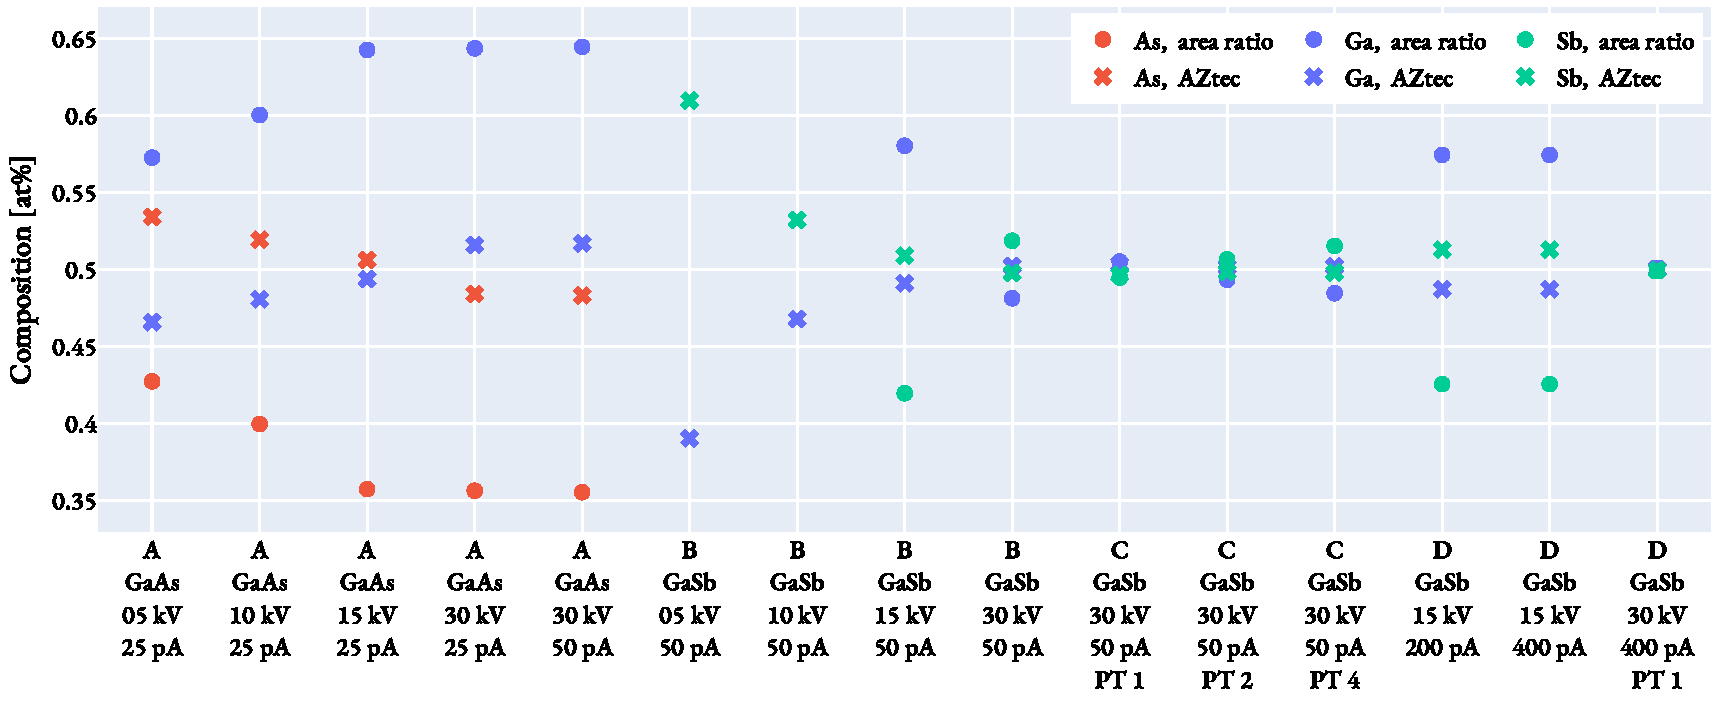
\includegraphics[width=0.99\linewidth]{figures/results/initial_quantification.pdf}
    \caption{
        Initial quantification results in at\%.
        The X markers are the quantification from AZtec.
        The circle markers are the quantification from the area ratio, without corrections.
        The group, specimen, $E_0$, $i_b$, and PT are shown on the x-axis.
        The spectra without noted PT are taken with PT 6.
        The same data is tabulated in \cref{tab:results:initial_quantification}.
    }
    \label{fig:results:initial_quantification}
\end{figure}

\ton{Are the next three paragraphs too much discussion?}

% comment on the severely poor results from GaAs at 5 kV
The GaSb spectrum at 5 kV is poorly quantified, both by AZtec and by the area ratio.
AZtec is quantifying the 5 kV GaSb spectrum with the Ga L$\alpha$ and Sb M$\eta$ peaks.
Sb M$\eta$ is around 0.4 keV, and at such low energy the absorption is high.
AZtec overestimates the absorption of the Sb M$\eta$ peak, and the result is a 60:40 composition.
The Sb M$\eta$ peak is not available in HyperSpy, so the area ratio is done with the Sb L$\alpha$ peak.
The overvoltage on Sb L$\alpha$ in the the 5 kV spectrum is below 1.4, while the overvoltage on the Ga L$\alpha$ is above 4.5, which results in a severely underestimated Sb content with the area ratio.
% TODO discussion: quantification on low kV of Sb and similar elements with L-peaks between 3 and 4 keV is hard. Have to do something very clever, but what?


% What corrections are needed for the area ratio?
\cref{tab:results:initial_quantification} and \cref{fig:results:initial_quantification} show that the need for corrections are varying with both specimen and acquisition parameters.
% GaAs
Different $i_b$ are not affecting the correction needs much, but the $E_0$ is.
All the GaAs spectra need corrections which increase the weight of As.
AZtec have applied corrections to the GaAs spectra, where the results are pushing As too high at 5 kV and 10 kV, and not high enough at 30 kV.
The 15 kV GaAs corrections done by AZtec on GaAs is good, resulting at 50.6:49.4.
% TODO discuss: the need to increase the weight of As is due to absoprtion of As X-rays is Ga.
% GaSb
The corrections needed in the GaSb spectra are not as clear as for GaAs.
The 30 kV GaSb spectra appears to require little corrections, and have good results with the area ratio.
The 15 kV and 10 kV spectra of GaSb need corrections to increase the weight of Sb.
The GaSb 15 kV and 10 kV spectra are quantified with Ga L$\alpha$ and Sb L$\alpha$.
% The intensity in the Sb L$\alpha$ peak in the 15 kV and 10 kV spectrum are too low, compared to the Ga L$\alpha$ peak.
AZtec have corrected the 15 kV compositions well, and semi-well for the 10 kV composition.
% TODO discuss: the need to increase the weight of Sb. The absorption should be stronger of Ga La, so this is not the reason. Probably a Z effect. Also overvoltage. Maybe omega.
Correction factors are presented in \cref{results:matrix_corrections}.

\brynjar{Move to disussion:
    "
    Since the absorption should be stronger of the Ga L$\alpha$ peak than the Sb L$\alpha$ peak, the absorption should not be the reason for the low Sb content.
    The low Sb content in the 15 kV and 10 kV spectra can be due to the overvoltage differences.
    Ga L$\alpha$ has overvoltage $U = 15/1.1 = 13.6$, and Sb L$\alpha$ has $U = 15/3.6 = 4.2$ at 15 kV.
    From the estimated ionization cross-section as a function of overvoltage, seen in \cref{fig:PAP:ionization_cross_section}, the maximum $Q(U)$ is at $U = 3.4$.
    Thus, the overvoltage at 15 kV should not be the reason for the low Sb content.
    % TODO discuss: the reason for the low Sb content at 15 kV is not the overvoltage, but something else.
    The different intensities are thus probably an effect of different Z. This should be treated somewhat by the PAP method.
    "}






\subsubsection*{Quantification of SEM data, pretended to be TEM data}

% Quantification while treating the specimen as a TEM specimen.
Quantification of the spectra was also done pretending that the specimen was a TEM specimen, both in AZtec and HyperSpy.
This is done in AZtec with the "TEM setting", which gives composition and calculated k-factors.
The calculated k-factors were taken and used with the Cliff-Lorimer method in HyperSpy, which gives composition.
In HyperSpy, the quantification was done with and without the TEM absorption corrections.
For the absorption corrections, four different thicknesses were used: 100nm, 1000 nm, 10000 nm, and 100000 nm.
As the results were poor, they are only commented on briefly in the text below.

% AZtec TEM setting
The AZtec TEM setting results on the SEM specimen yielded poor results.
The 5 kV GaAs spectrum and the 30 kV GaSb spectra was quantified at a 45:55 ratio.
The remaining spectra were quantified around a 70:30 ratio.


% HyperSpy Cliff-Lorimer
The Cliff-Lorimer TEM quantification method in HyperSpy yielded poor results too.
Adding absorption corrections through the Cliff-Lorimer method did not improve the results.
The implemented absorption correction is a part of the Cliff-Lorimer method, and thus made for TEM specimens.
The low voltage spectra were quantified at a 70:30 ratio or worse.
% todo discuss: probably due to TEM being high HT.
The 30 kV spectra were quantified at a 55-60:45-40 ratio, and the absorption corrections improved the results somewhat with t = 1000 nm for GaSb and t = 10000 nm for GaAs.
% todo discuss: the absorption corrections in the CL method, as used briefly in this work, does not give a general improvement.




\subsection{Matrix corrections}
\label{results:matrix_corrections}



\subsubsection{ZAF absorption corrections}
\label{results:matrix_corrections:ZAF}

The ZAF absorption corrections were done with \cref{eq:theory:quantitative:absorption}. %, and the results are presented in \cref{tab:results:ZAF_corrections_factors} and \cref{tab:results:ZAF_corrections_compositions}.
The calculated maximum electron range $t$ is presented in \cref{tab:results:ZAF_corrections_range_t}.
The parameters are line, elements, $\mu_\rho$, $\rho$, $E_0$, assumed atomic fraction, TOA, and maximum electron range $t$.
To calculate the absorption correction factors, $t$ is divided by 2, 3, and 4 to get different approximations for the average depth of origin of the X-rays.
The calculated absorption correction factors are presented in \cref{tab:results:ZAF_corrections_factors}.
The corrected compositions are presented in \cref{tab:results:ZAF_corrections_compositions}.

\ton{Can I drop the GaSb absorption corrections? They only make the results worse.}

\ton{TODO: the densities are not the same as stated on Wikipedia.}


\begin{table}[htbp]
    \begin{center}
        \caption{
            Parameters for calculating the absorption correction factors.
            The calculated maximum electron ranges, $t$, used calculated using HyperSpy, see \cref{todo}.
            %
        }
        %\renewcommand*{\arraystretch}{1.4}
        \label{tab:results:ZAF_corrections_range_t}
        \begin{tabular}{rrrrr}
            \hline
            \textbf{Parameter} & \textbf{GaAs value} & \textbf{GaSb value} \\
            \hline
            $\rho$             & 5.81 g/cm$^3$       & 6.41 g/cm$^3$       \\
            TOA                & 35\textdegree       & 35\textdegree       \\
            $t$ at 30 kV       & 7.96 um             & 7.22 um             \\
            $t$ at 15 kV       & 2.5 um              & 2.27 um             \\
            $t$ at 10 kV       & 1.27 um             & 1.15 um             \\
            $t$ at 5 kV        & 0.4 um              & 0.36 um             \\
            \hline
        \end{tabular}
    \end{center}
\end{table}

\begin{table}[phtb]
    \begin{center}
        \caption{
            Absorption correction factors from the ZAF method used.
            The absorption correction factors are in the three rightmost colums, idicated by "A t/x", where x is the number that the maximum electron range is divided by.
            Similar specimen, line, and $E_0$ have the same A, thus some of the duplicated spectra are removed.
        }
        %\renewcommand*{\arraystretch}{1.4}
        \label{tab:results:ZAF_corrections_factors}
        \begin{tabular}{rrrrrr}
            \hline
            \textbf{ Group} & \textbf{Line} & \textbf{$E_0$} & \textbf{A with t/2} & \textbf{A with t/3} & \textbf{A t/4} \\
            \emph{}         & \emph{}       & \emph{[kV]}    & \emph{}        & \emph{}        & \emph{}        \\
            \hline
            A               & As L$\alpha$  & 5              & 1.54           & 1.33           & 1.24           \\
            A               & Ga L$\alpha$  & 5              & 1.18           & 1.12           & 1.09           \\
            A               & As L$\alpha$  & 10             & 3.93           & 2.49           & 1.98           \\
            A               & Ga L$\alpha$  & 10             & 1.69           & 1.42           & 1.30           \\
            A               & As L$\alpha$  & 15             & 14.79          & 6.02           & 3.85           \\
            A               & Ga L$\alpha$  & 15             & 2.80           & 1.99           & 1.67           \\
            A               & As K$\alpha$  & 30             & 1.33           & 1.21           & 1.15           \\
            A               & Ga K$\alpha$  & 30             & 1.11           & 1.07           & 1.05           \\
            %A&As K$\alpha$&30&1.33&1.21&1.15\\
            %A&Ga K$\alpha$&30&1.11&1.07&1.05\\
            \hline
            B               & Ga L$\alpha$  & 5              & 1.73           & 1.44           & 1.32           \\
            B               & Sb L$\alpha$  & 5              & 1.05           & 1.03           & 1.03           \\
            B               & Ga L$\alpha$  & 10             & 5.72           & 3.20           & 2.39           \\
            B               & Sb L$\alpha$  & 10             & 1.17           & 1.11           & 1.08           \\
            B, D            & Ga L$\alpha$  & 15             & 31.00          & 9.87           & 5.57           \\
            B, D            & Sb L$\alpha$  & 15             & 1.37           & 1.23           & 1.17           \\
            B, C, D         & Ga K$\alpha$  & 30             & 1.33           & 1.21           & 1.16           \\
            B, C, D         & Sb L$\alpha$  & 30             & 2.71           & 1.94           & 1.65           \\
            % \hline          &               &                &                &                &                \\
            %C&Ga K$\alpha$&30&1.33&1.21&1.16\\
            %C&Sb L$\alpha$&30&2.71&1.94&1.65\\
            %C&Ga K$\alpha$&30&1.33&1.21&1.16\\
            %C&Sb L$\alpha$&30&2.71&1.94&1.65\\
            %C&Ga K$\alpha$&30&1.33&1.21&1.16\\
            %C&Sb L$\alpha$&30&2.71&1.94&1.65\\
            % \hline          &               &                &                &                &                \\
            %D&Ga K$\alpha$&30&1.33&1.21&1.16\\
            %D&Sb L$\alpha$&30&2.71&1.94&1.65\\
            %D&Ga L$\alpha$&15&31.00&9.87&5.57\\
            %D&Sb L$\alpha$&15&1.37&1.23&1.17\\
            %D&Ga L$\alpha$&15&31.00&9.87&5.57\\
            %D&Sb L$\alpha$&15&1.37&1.23&1.17\\
            %
            %E&Map&&&&\\
            %E&Map&&&&\\
            %&&&&&\\
            \hline
        \end{tabular}
    \end{center}
\end{table}

\newgeometry{top=2cm} % change the margins to fit the table.
\begin{table}[phtb]
    \begin{center}
        \caption{
            Compositions from the intensity ratio method with absorption corrected intensities. The uncorrected at.\% value is tabulated for reference.
            See \cref{tab:results:ZAF_corrections_factors} for the correction factors.
            Average numbers are given in \cref{tab:results:ZAF_corrections_compositions_stats}.
            Each spectrum has two lines in the table.
        }
        %\renewcommand*{\arraystretch}{1.4}
        \label{tab:results:ZAF_corrections_compositions}
        \begin{tabular}{rrrrrrrr}
            \hline
            \textbf{Groups} & \textbf{Line} & \textbf{$E_0$} & \textbf{$i_b$} & \textbf{Uncorr. at.\%} & \textbf{at.\% with r/2} & \textbf{at.\% with r/3} & \textbf{at.\% with r/4} \\
            \emph{}         & \emph{}       & \emph{[kV]}    & \emph{[pA]}    & \emph{}                & \emph{}                 & \emph{}                 & \emph{}                 \\
            \hline
            A               & As L$\alpha$  & 5              & 25             & 43                     & 48                      & 46                      & 45                      \\
            A               & Ga L$\alpha$  & 5              & 25             & 57                     & 52                      & 54                      & 55                      \\
            A               & As L$\alpha$  & 10             & 25             & 40                     & 58                      & 52                      & 49                      \\
            A               & Ga L$\alpha$  & 10             & 25             & 60                     & 42                      & 48                      & 51                      \\
            A               & As L$\alpha$  & 15             & 25             & 36                     & 71                      & 60                      & 54                      \\
            A               & Ga L$\alpha$  & 15             & 25             & 64                     & 29                      & 40                      & 46                      \\
            A               & As K$\alpha$  & 30             & 25             & 36                     & 39                      & 38                      & 37                      \\
            A               & Ga K$\alpha$  & 30             & 25             & 64                     & 61                      & 62                      & 63                      \\
            A               & As K$\alpha$  & 30             & 50             & 36                     & 39                      & 38                      & 37                      \\
            A               & Ga K$\alpha$  & 30             & 50             & 64                     & 61                      & 62                      & 63                      \\
            \hline
            B               & Ga L$\alpha$  & 5              & 50             & 97                     & 98                      & 98                      & 98                      \\
            B               & Sb L$\alpha$  & 5              & 50             & 3                      & 2                       & 2                       & 2                       \\
            B               & Ga L$\alpha$  & 10             & 50             & 75                     & 93                      & 89                      & 86                      \\
            B               & Sb L$\alpha$  & 10             & 50             & 25                     & 7                       & 11                      & 14                      \\
            B               & Ga L$\alpha$  & 15             & 50             & 58                     & 97                      & 91                      & 86                      \\
            B               & Sb L$\alpha$  & 15             & 50             & 42                     & 3                       & 9                       & 14                      \\
            B               & Ga K$\alpha$  & 30             & 50             & 48                     & 32                      & 37                      & 40                      \\
            B               & Sb L$\alpha$  & 30             & 50             & 52                     & 68                      & 63                      & 60                      \\
            \hline
            C               & Ga K$\alpha$  & 30             & 50             & 48                     & 32                      & 37                      & 40                      \\
            C               & Sb L$\alpha$  & 30             & 50             & 52                     & 68                      & 63                      & 60                      \\
            C               & Ga K$\alpha$  & 30             & 50             & 49                     & 33                      & 38                      & 41                      \\
            C               & Sb L$\alpha$  & 30             & 50             & 51                     & 67                      & 62                      & 59                      \\
            C               & Ga K$\alpha$  & 30             & 50             & 51                     & 34                      & 39                      & 42                      \\
            C               & Sb L$\alpha$  & 30             & 50             & 49                     & 66                      & 61                      & 58                      \\
            \hline
            D               & Ga L$\alpha$  & 15             & 200            & 57                     & 97                      & 91                      & 86                      \\
            D               & Sb L$\alpha$  & 15             & 200            & 43                     & 3                       & 9                       & 14                      \\
            D               & Ga L$\alpha$  & 15             & 400            & 57                     & 97                      & 91                      & 86                      \\
            D               & Sb L$\alpha$  & 15             & 400            & 43                     & 3                       & 9                       & 14                      \\
            D               & Ga K$\alpha$  & 30             & 400            & 50                     & 33                      & 39                      & 41                      \\
            D               & Sb L$\alpha$  & 30             & 400            & 50                     & 67                      & 61                      & 59                      \\
            %
            %E&Map&&&&&&\\
            %E&Map&&&&&&\\
            %&&&&&&&\\
            \hline
        \end{tabular}
    \end{center}
\end{table}
\restoregeometry % put the margins back to normal





\subsubsection{XPP/PAP corrections}
\label{results:matrix_corrections:XPP}



% Old
% % % The model lines

\begin{table}[p]
    \centering
    \caption{
        The lines in the HyperSpy models for the GaAs sample, when As and Ga are added as elements.
        The dashed lines are the lines that are not used in the model, because of low overvoltage.
        HyperSpy differentiates between "X-ray lines" and "Family lines", where the first are the alpha lines of the element.
    }
    \label{tab:results:model_lines}
    \begin{tabular}{c|ccccccccccc}
        X-ray lines  &       &        &       &       &        &       &        &       &       &        \\
        % Model        &       &        &       &       &        &       &        &       &       &        \\
        30 kV        & As Ka & As La  & Ga Ka & Ga La &        &       &        &       &       &        \\
        15 kV        & As Ka & As La  & Ga Ka & Ga La &        &       &        &       &       &        \\
        10 kV        & ----- & As La  & Ga Ka & Ga La &        &       &        &       &       &        \\
        5            & ----- & As La  & ----- & Ga La &        &       &        &       &       &        \\
        \hline
        Family lines &       &        &       &       &        &       &        &       &       &        \\
        30 kV        & As Kb & As Lb1 & As Ln & As Ll & As Lb3 & Ga Kb & Ga Lb1 & Ga Ln & Ga Ll & Ga Lb3 \\
        15 kV        & As Kb & As Lb1 & As Ln & As Ll & As Lb3 & Ga Kb & Ga Lb1 & Ga Ln & Ga Ll & Ga Lb3 \\
        10 kV        & ----- & As Lb1 & As Ln & As Ll & As Lb3 & ----- & Ga Lb1 & Ga Ln & Ga Ll & Ga Lb3 \\
        5  kV        & ----- & As Lb1 & As Ln & As Ll & As Lb3 & ----- & Ga Lb1 & Ga Ln & Ga Ll & Ga Lb3
    \end{tabular}
\end{table}
% \begin{table}[p]
    \centering
    \caption{
        The estimated FWHM of Mn K$\alpha$ with different reference lines.
        When using 'all\_alpha', the alphabetically first line is used as reference.
        That is, for 30 and 15 kV, As K$\alpha$ is used as reference.
        For 10 and 5 kV, As L$\alpha$ is used as reference.
        The original resolution is from the instrument software.
    }
    \label{tab:results:estimated-FWHM}
    \begin{tabular}{ccccc}
        Reference line      & 30 kV & 15 kV & 10 kV & 5 kV  \\
        \hline
        original resolution & 130.0 & 130.0 & 130.0 & 130.0 \\
        \verb|'all_alpha'|  & 138.3 & 148.8 & 132.0 & 132.2 \\
        As Ka               & 137.9 & 146.4 & nan   & nan   \\
        As La               & 130.0 & 130.4 & 131.9 & 132.1 \\
        Ga Ka               & 132.9 & 131.7 & 668.3 & nan   \\
        Ga La               & 129.7 & 130.9 & 127.4 & 130.8
    \end{tabular}
\end{table}
% \subsection{Energy resolution}
% \label{results:resolution}